The characteristics of the nearest neighbors of each record can provide useful insight into the nature of clustering of data.

\subsection{Variation of distribution for the first four nearest neighbors}
The change in the distribution of the distance of nearest neighbor with the class and neighbor position, is shown in Fig:11 and Fig:12. The method to generate the plot is as follows - 
\begin{figure}[h]
		\label{fig:proximity-distribution-class1}
		\caption{Distribution of distances of the first 4 nearest neighbors for records in class '$<=$50K'}
		\centering
		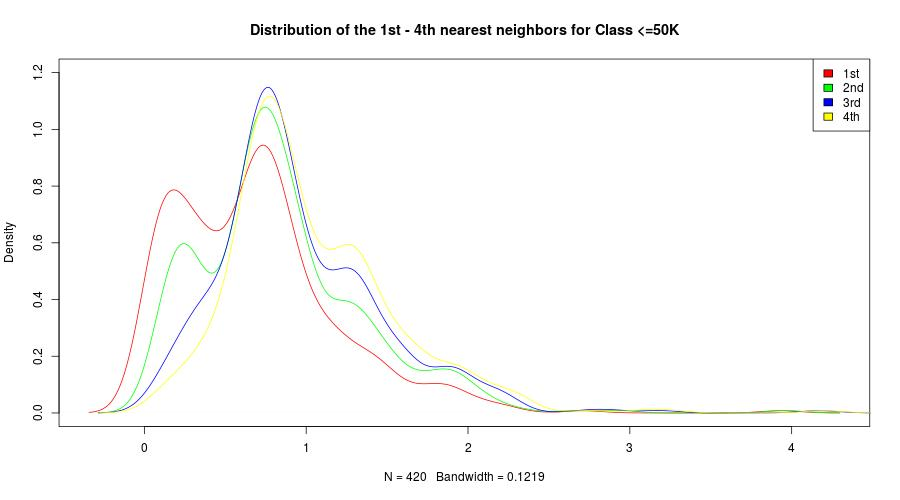
\includegraphics[width=0.5\textwidth]{images/proximity-distribution-class1.jpg}
\end{figure}
\begin{figure}[h]
		\label{fig:proximity-distribution-class2}
		\caption{Distribution of distances of the first 4 nearest neighbors for records in class '$>$50K'}
		\centering
		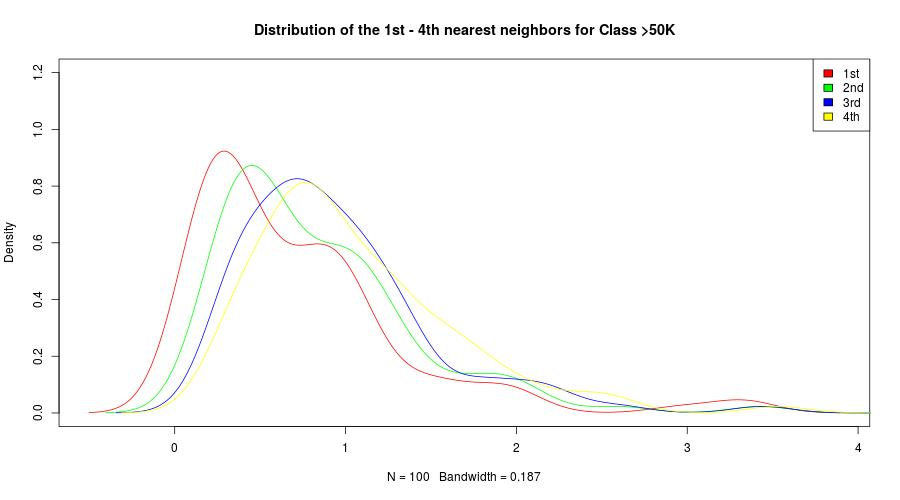
\includegraphics[width=0.5\textwidth]{images/proximity-distribution-class2.jpg}
\end{figure}

\begin{enumerate}
\item The dataset was divided in to two by class.
\item For each element in each class, the first four nearest neighbors and their distances were computed.
\item The distributions were plotted for each class separately. The distance of the neighbor increases along the positive x-axis, while the y-axis represents the number density. In mathematical terms, the number of records having a neighbor between distances $x$ and $x+dx$ is given by $ydx$.
\end{enumerate}

For the lower income class (Fig:11) it can be seen that the distributions for the four nearest neighbors has two peaks. The first peak is at 0.2-0.3 and the second peak is at 0.8 - 0.9. These two peaks represent two clusters. In the first cluster the points belonging to lower income class are clustered close together with most of the points having their first neighbor at 0.2-0.3. The second cluster is larger but sparse. The first neighbor in this cluster is at 0.8-0.9 for most of the points. Also the the distributions move rightward as we move towards the fourth neighbor. However the change is not so much for the third and fourth nears neighbors. This indicates a saturation of some kind.\\

For the upper income class (Fig:12) the four distributions are different from the lower income class. There is only one peak which gradually widens as we move to distributions for higher number of neighbors. This indicates the presence of only one cluster in the upper income class. Also this data is more closely packed as compared to lower income dataset. This indicates that the people in upper income bracket have much less variation in their attributes as compared to people in lower income category.

\subsection{Variation of distribution of number of neighbors in a 1 unit ball}
The variation of distribution of the number records in 1 unit proximity of a record is plotted in Fig:\ref{fig:numberof-neighbors-class1} and Fig:\ref{fig:numberof-neighbors-class2}. The method to generate the plot is as follows - 

\begin{figure}[h]
		\label{fig:numberof-neighbors-class1}
		\caption{Distribution of distances of the first 4 nearest neighbors for records in class '$<=$50K'}
		\centering
		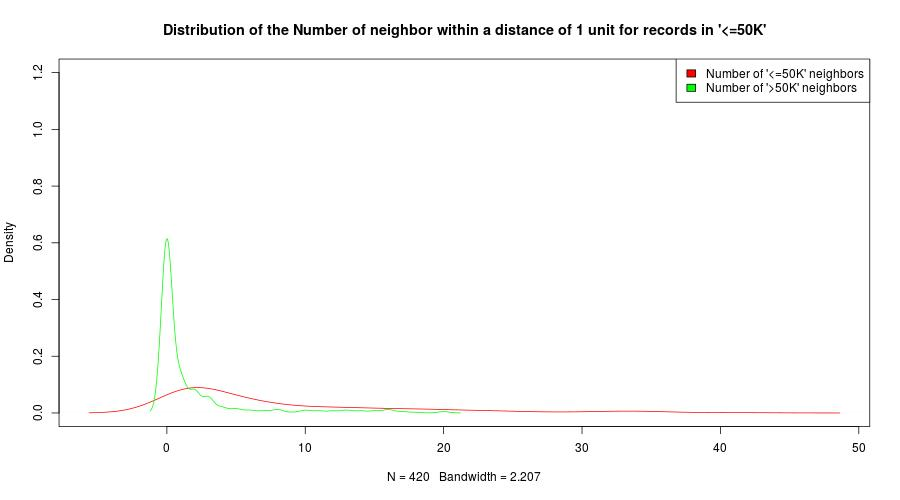
\includegraphics[width=0.5\textwidth]{images/numberof-neighbors-class1.jpg}
\end{figure}
\begin{figure}[h]
		\label{fig:numberof-neighbors-class2}
		\caption{Distribution of distances of the first 4 nearest neighbors for records in class '$>$50K'}
		\centering
		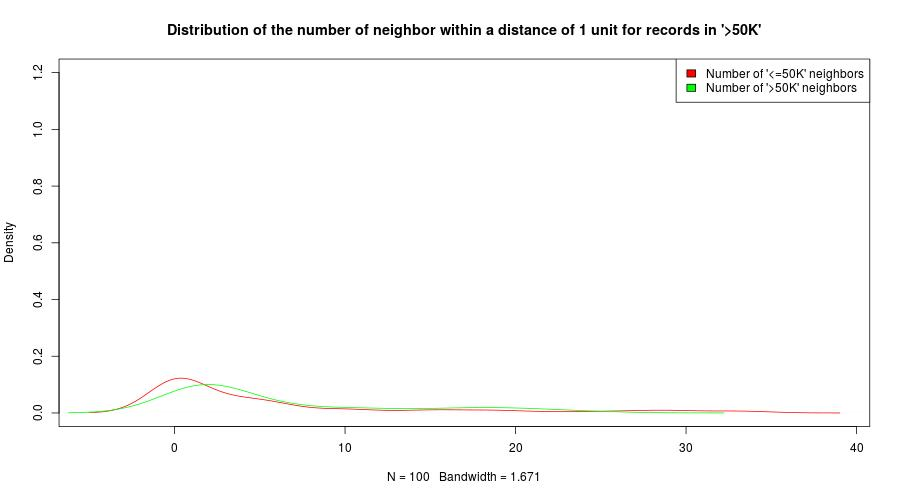
\includegraphics[width=0.5\textwidth]{images/numberof-neighbors-class2.jpg}
\end{figure}

\begin{enumerate}
\item The dataset was divided in to two according to the class.
\item For records of each class the number of neighbors in a unit ball were calculated. These calculation were made across the classes and with in the classes.
\item Each plot has the number of neighbors on the x-axis and the density on the y-axis.
\item Two distributions were obtained for each of the classes. For the upper income class the distribution in red shows the distribution of number of lower income people in a unit ball neighborhood. The green line in the same plot shows the distribution of other upper income people in the same sized neighborhood. The other plot similarity shows the two distributions for the lower income people.
\end{enumerate}

In the plot for lower income people (Fig:13) there is a massive peak in the green line. The peak is very close to zero. This means that for large number of lower income people there close to 0 or 1 upper income points in their neighborhood. The red graph has a small bump that is spread over a number of values from 0 to 4, indicating that for a large number of points in lower income class the space is sparsely populated with 1-4 neighbors. The tail of green class extends to 30, which indicates the presence of outliers in the lower income class that is deep inside the upper income class territory. The tail of the red graph indicates that the there are over 30-40 records in lower income category that are more or less the same.\\
The distributions are a little different for the records in upper income category. The red graph has a peak closer to zero. So many of the upper income records do have a lower income record in their neighborhood. Instead they have each other in their neighborhood. This is indicated by the green graph which has a peak over 1. The two peaks are not very pronounced, hence it can be concluded that the many of the upper income records are rather spread out and are at times quite close to the lower income records.\\

This analysis gives a good idea of what 'k' to choose for a k-NN classifier. Since most records have 2 or more of the same kind of record in their neighborhood, it can be expected that a k-NN with k=2 will give a good classification results.\\
